\chapter{Electromagnetic Waves}

Sound is a compression wave -- to travel, it needs a medium to
compress: air, water, etc. (Regardless of what you have seen in
movies, sound does not travel through a vacuum)

Light is an electromagnetic wave -- it causes fluctuations in the
electric and magnetic fields that are everywhere. It can cross a
vacuum, as it does to reach us from the sun.

Electromagnetic waves travel at about 300 million meters per second in a
vacuum. The waves travel slower through things. For example, an
electromagnetic wave travels at 225 million meters in water.

Electromagnetic waves come in different frequencies. For example, the
light coming out of a red laser pointer is usually about $4.75 \times
10^{14}$ Hz.  The wifi data sent by your computer is carried on an
electromagnetic wave too. It is usually close to $2.4 \times 10^6$ Hz
or $5 \times 10^6$ Hz.

Because we know how fast the waves are moving, we sometimes talk about
their wavelengths instead of their frequencies.  The light coming out
of a laser pointer is $300 \times 10^6 / 4.76 \times 10^{14} = 630
\times 10^{-9}$ m, or 630 nm.

\begin{Exercise}[title={Wavelengths}, label=wave_length_green]

  A green laser pointer emits light at $5.66 \times
10^{14}$ Hz. What is its wavelength in a vacuum?
  
\end{Exercise}
\begin{Answer}[ref=wave_length_green]
$$\frac{300 \times 10^6}{5.66 \times 10^{14}} = 530 \times 10^{-9} = 530\text{ nm}$$
\end{Answer}

We have given names to different ranges of the electromagnetic spectrum:

\begin{tabular}{r | l | l}
  Name & Hertz & Meters \\
  \hline
Gamma rays  & $  \times 10^{}$ &$ \times 10^{}$\\
X-rays  & $ \times 10^{}$&$ \times 10^{}$\\
Ultraviolet  & $ \times 10^{}$&$ \times 10^{}$\\
Blue & $ \times 10^{}$&$ \times 10^{}$\\
Red  & $ \times 10^{}$&$ \times 10^{}$\\
Infrared  & $ \times 10^{}$&$ \times 10^{}$\\
Microwaves  & $ \times 10^{}$&$ \times 10^{}$\\
Radio waves  & $ \times 10^{}$&$ \times 10^{}$\\
\end{tabular}

(You may have heard of ``cosmic rays'' and wonder why they are
not listed in this table. Cosmic rays are actually the nuclei of atoms
that have been stripped of their electron cloud. These particles come
flying out of the sun at very high speeds. They were originally
thought to be electromagnetic waves, and they were mistakenly named
``rays''.)

In general, the lower frequency the wave is, the better it passes
through a mass.  A radio wave, for example, can pass through the walls
of your house, but visible light cannot.  The people who designed the
microwave oven, chose the frequency of 2.45 GHz because the energy
from those waves tended to get absorbed in the first few inches of
food that it passed through.

\section{The greenhouse effect}

Humans have dug up a bunch of long carbon-based molecules (like oil
and coal) and burned them, releasing large amounts of $CO_2$ into the
atmosphere. It is not obvious why that has made the planet warmer. The
answer is electromagnetic waves.

A warm object gives off infrared electromagnetic waves. That's why,
for example, motion detectors in security systems are actually
infrared detectors: even in a dark room, your body gives off a lot of
infrared radiation.

You may have heard of ``heat-seeking missiles.'' These are more
accurately called ``Infrared homing missiles'' because they follow
objects giving off infrared radiation -- hot things like jet engines.

The sun beams a lot of energy to our planet in the form of
electromagnetic radiation: visible light, infrared, ultraviolet. (How
much? At the top of the atmosphere directly facing the sun, we get
1,360 watts of radiation per square meter. That is a lot of power!)

Some of that radiation just reflects back into space.  23\% is
reflected by the clouds and the atmosphere, 7\% makes it all the way
to the surface of the planet and is reflected back into space.

The other 71\% is absorbed: 48\% is absorbed by the surface and 23\%
is absorbed by the atmosphere. All of that energy warms the planet and
the atmosphere so that it gives off infrared radiation. The planet
lives in equilibrium: The infrared radiation leaving our atmosphere is
exactly the same amount of energy as that 71\% of the radiation that
it absorbs.

(If the planet absorbs more energy than it releases, the planet gets
hotter.  Hotter things release more infrared. When the planet is in
equilibrium again, it stops getting hotter.)

So what is the problem with $CO_2$ and other large molecules in the
atmosphere? They absorb the infrared radiation instead of letting it
escape into space. Thus the planet must be hotter to maintain
equilibrium.

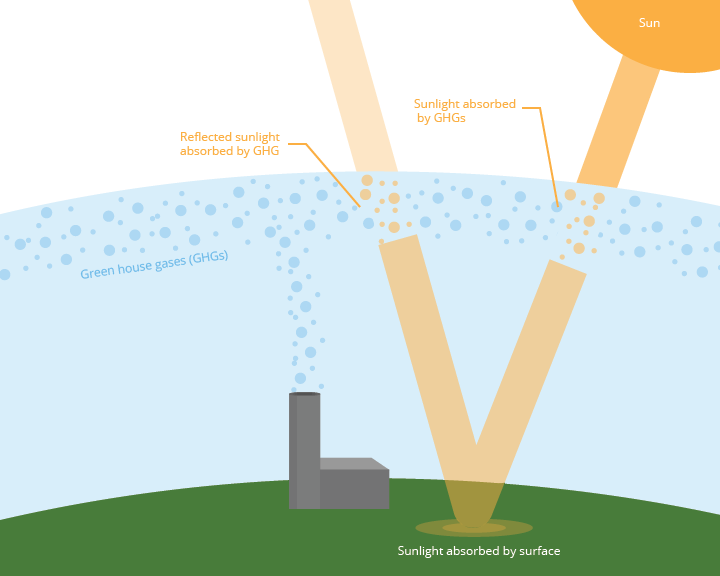
\includegraphics[width=1\textwidth]{ghgEffect.png}

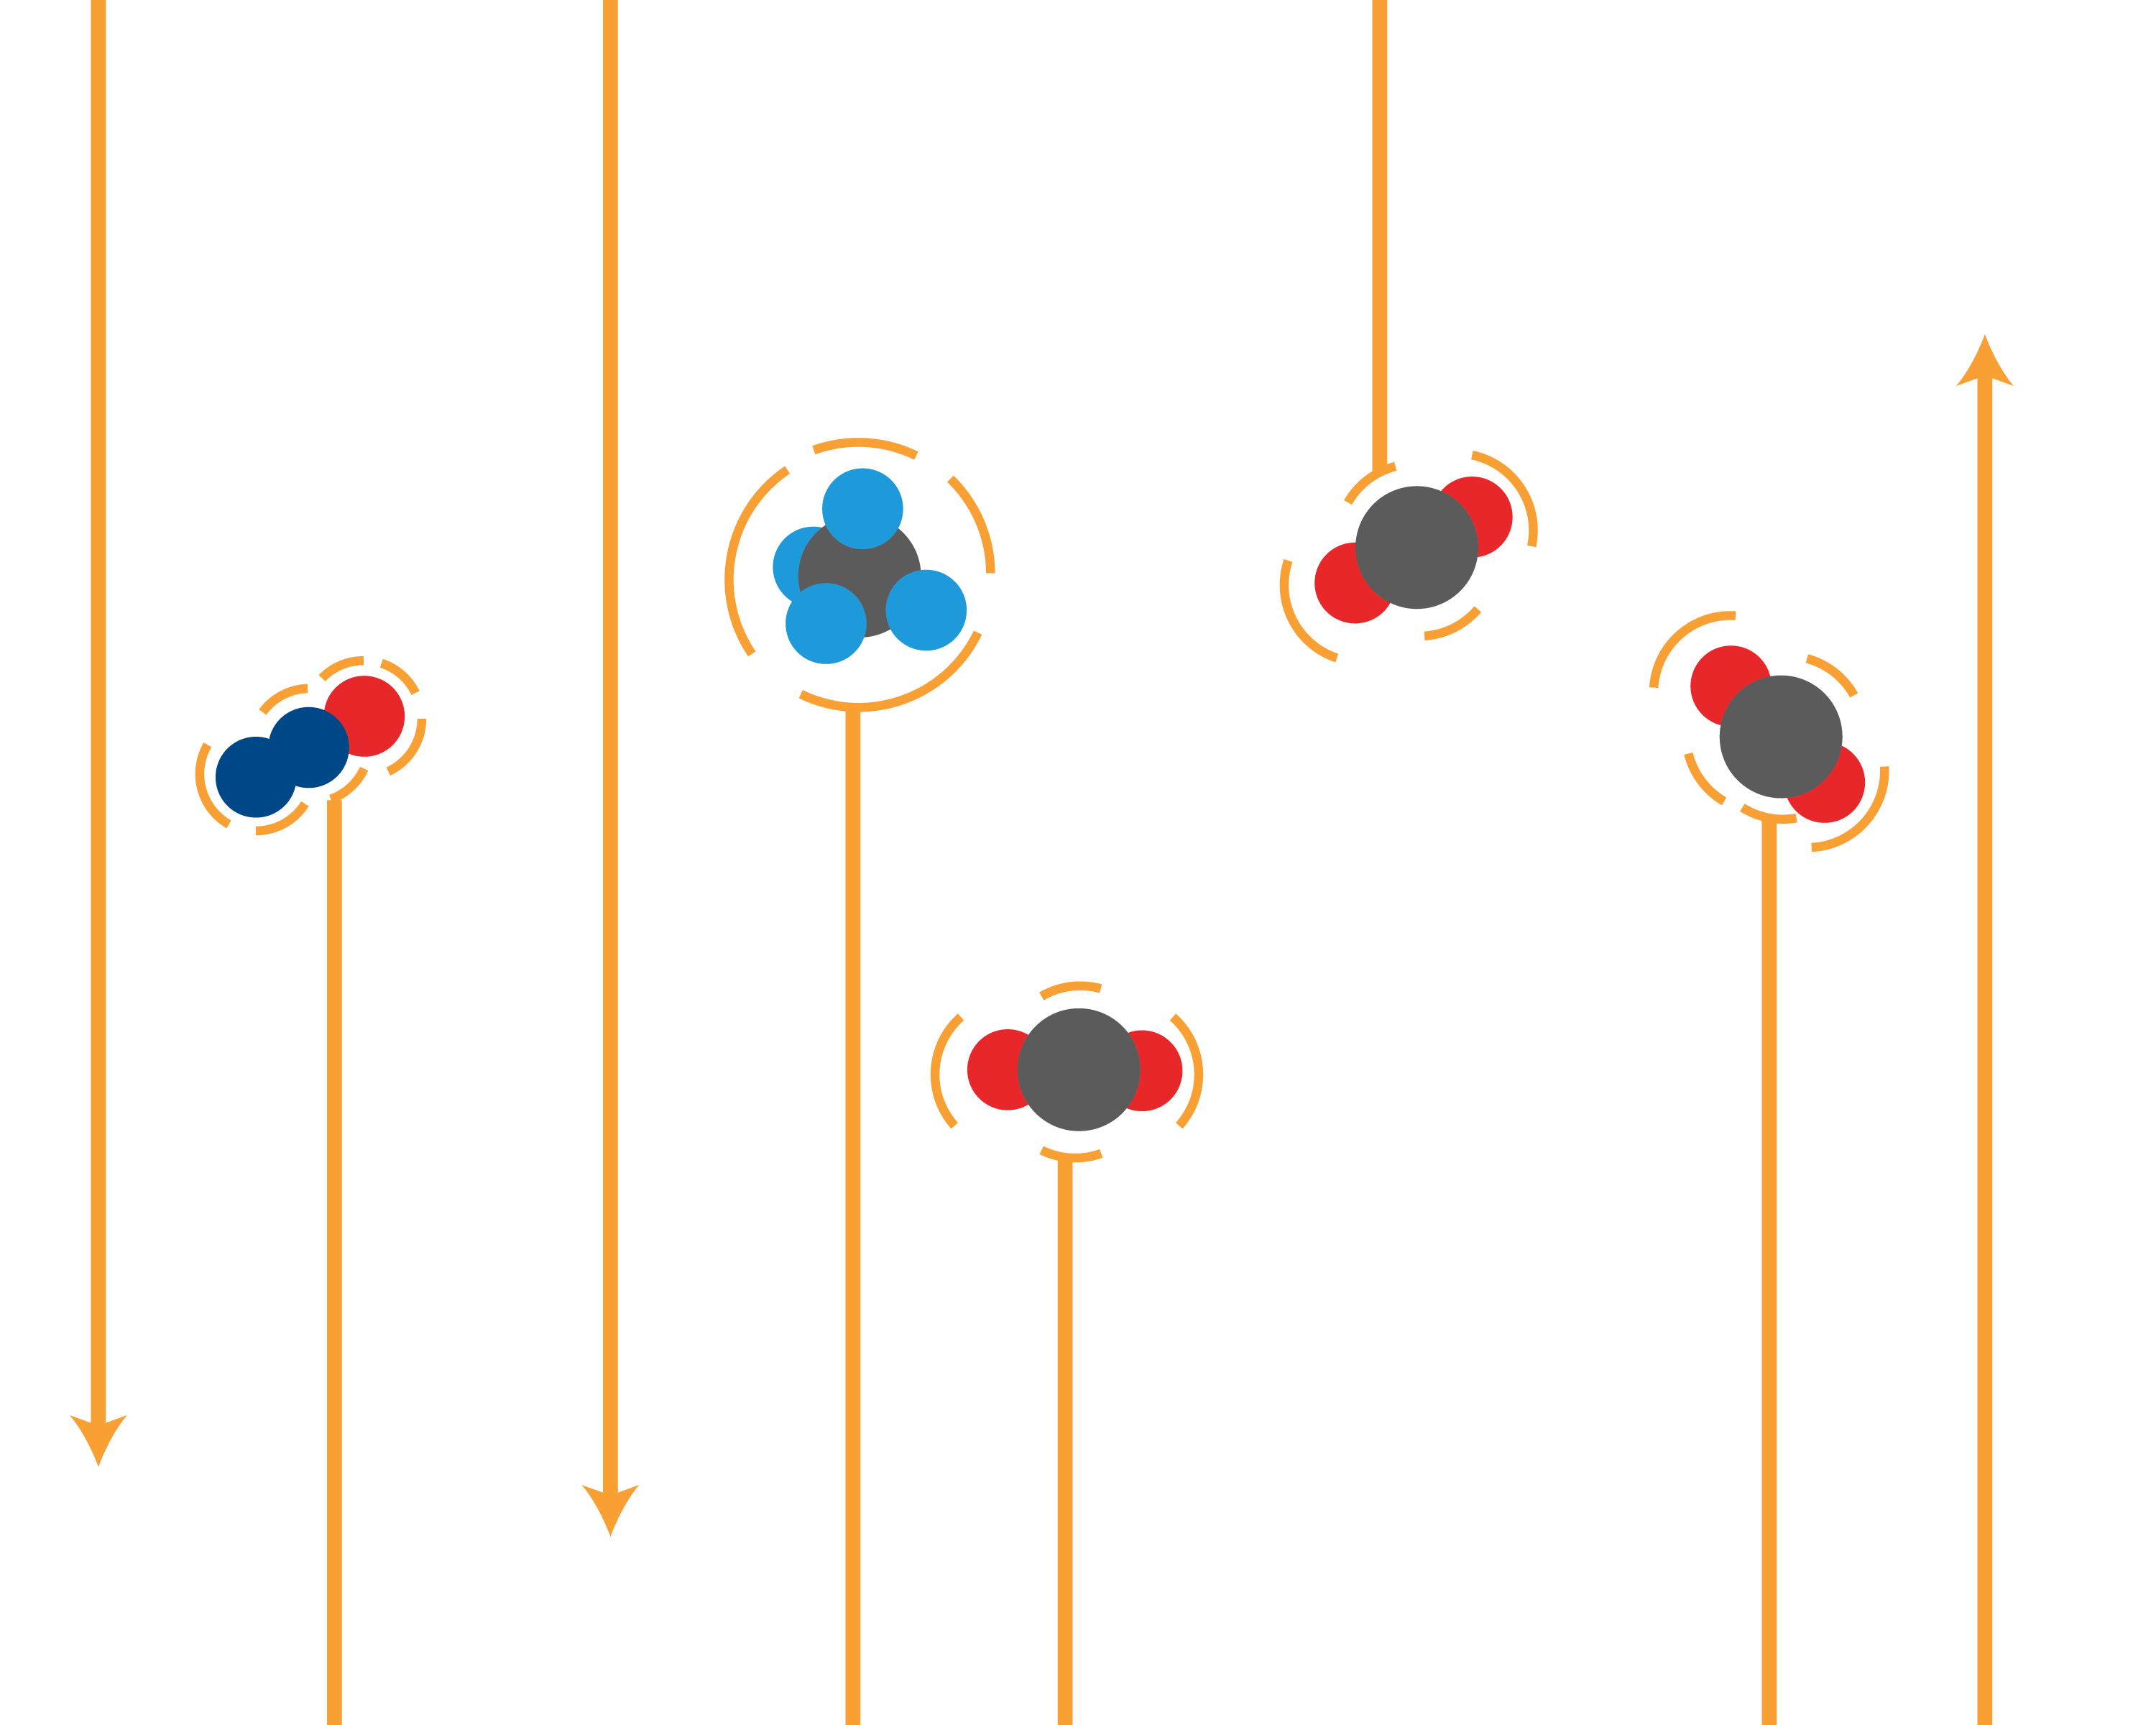
\includegraphics[width=.5\textwidth]{ghgClose.png}

The planet is getting hotter, and it is creating a multitude of
problems:
\begin{itemize}
\item Weather patterns are changing, which leads to extreme floods and
  droughts.
  
\item Ice and snow in places like Greenland are melting and flowing
  into the oceans. This is raising sea-levels.
  
\item Biomes with biodiversity are resilient. Rapidly changing climate
  is destroying biodiversity everywhere, which is making these ecosystems
  very fragile.
  
\item In many places, permafrost, which has trapped large amounts of
  methane in the ground for millenia, is melting.
\end{itemize}

That last item is particularly scary because methane is a large gas
molecule -- it absorbs even more infrared radiation than $CO_2$. As it is
escapes the permafrost, the problem will get worse.

Scientists are working on four kinds of solutions:
\begin{itemize}
  \item \textbf{Stop increasing the amount of greenhouse gases in our
    atmosphere.} It is hoped that non-carbon based energy systems like
    solar, wind, hydroelectric, and nuclear could let us stop burning
    carbon. Given the methane already being released, it maybe too
    late for this solution to work on its own.

  \item \textbf{Take some of greenhouse gases out of our atmosphere and
    sequester them somewhere.} The trunk of a tree is largely carbon
    molecules. When you grow a tree where there had not been one
    before, you are sequestering carbon inside the tree.  There are
    also scientists that are trying to develop process that pull
    greenhouse gases out of the air and turn them into solids.

  \item \textbf{Decrease the amount of solar radiation that is
    absorbed by our planet and its atmosphere.} Clouds reflect a lot of radiation back into
    space. Could we increase the cloudiness of our atmosphere? Or
    maybe  mirrors in orbit around our planet?

  \item \textbf{Adapt to the changing climate.} These scientists are
    assuming that global warming will continue, and are working to
    minimize future human suffering. How will we relocate a billion
    people as the oceans claim their homes?  When massive heat waves
    occur, how will we keep people from dying?  As biodiversity
    decreases, how can we make sure that species that are important to
    human existence survive?
    
\end{itemize}

What are the greenhouse gases and how much does each contribute to
keeping the heat from exiting to space?  These numbers are still being
debated, but this will give you a feel:
\begin{tabular}{c | c | c}
  Water vapor & $H_2O$ & 36 - 72 \% \\
  Carbon dioxide & $CO_2$ & 9 - 26 \% \\
  Methane & $CH_4$ & 4 - 9 \% \\
  Ozone & $O_3$ & 3 - 7 \%
\end{tabular}

Notice that while we talk a lot about carbon dioxide, the most
important greenhouse gas is actually water.  Why don't we talk about
it? Given the enormous surfaces of the oceans, it is difficult to
imagine any way to permanently decrease the amount of water in the
air. Also, a lot of water in the air is in the form of clouds that
help reflect radiation before it is absorbed.

